\documentclass[journal]{IEEEtran/IEEEtran}

\usepackage[utf8x]{inputenc}
\usepackage{cite}
\usepackage{hyperref}
\usepackage{url}
\usepackage{verbatim}
\usepackage{epstopdf}
\usepackage{amssymb}
\usepackage[pdftex]{graphicx}
\graphicspath{{img/}}
\DeclareGraphicsExtensions{.eps,.pdf,.png,.jpg,.jpeg}
\usepackage[cmex10]{amsmath}
\usepackage{array}

\usepackage{fancyvrb}
\DefineVerbatimEnvironment{code}{Verbatim}{fontsize=\small}


% correct bad hyphenation here
\hyphenation{op-tical net-works semi-conduc-tor}

\begin{document}
\title{Data Stream Analisys and Data Mining With Storm}

\author{Gregor~Majcen, Miha~Zidar}%
\markboth{MLDM Workshop, January~2013}{}
%\IEEEspecialpapernotice{(Invited Paper)}
\maketitle
\begin{abstract}
    Twitter Storm is a powerfull distributed real time data processing solution, with a wide range of usage. In this paper, we are going to take a look at how we can utilize Twitter Storms power for data mining on streams of data. The main focus of this paper is real time data processing and online data mining.
\end{abstract}

\begin{IEEEkeywords}
    online learning, continuous data, data mining, distributed systems, horizontal scaling, batch processing
\end{IEEEkeywords}

\IEEEpeerreviewmaketitle


\section{Introduction}
\IEEEPARstart{T}{oday} we're generating more information per second than ever before, and the amount of data produced is only increasing over time. Data on its own is not that useful for us, unless we can extract information from it and the speed of gathering that information is becomming more and more valuable. This is where the real time data processing comes in. Big companies like Twitter, Groupon, spider.io and others, are using Twitter Storm to provide a better user experience.\\

In the last few years data processing has come a long way with services like MapReduce, Amazon EMR, Hadoop, and related techologies. All of these were made to handle massive amounts of data, and they do that very affectively. But lately their weakness is showing in their lack of real time processing. Now speed is starting to be ever more important, to get ahead of competition. This is where Storm comes in. Unlike other solutions that work in "batch" mode, Storm is made so it can handle data streams. With that it's possible to get calculations done on tupples of data and have the results back in matter of seconds, insted of hours or even days. One valuable ability to have, with ever increasing data streams, is scalability. To be more precise, horizontal scalability, where if the data stream grows, we can simply add more nodes withought having to increase the speed of each individual node, and Twitter Storm prodvides that by running on top of Apache Zookeeper cluster.

We will begin by explaining what Storm is, how it works, and what it is used for. Then we shell slowly narow down all the Storm uses to the ones that become useful in datamining. We will show how a simple storm demo project, and discuss how these concepts can be applied to machine learning. At the end we will look at a practical machine learning algorithm running on Storm, then we'll take that knowlage to hypothesise a solution for the stock market prediction.

%\hfill mds%?
\hfill \today
\section{Twitter Storm}
Storm is a distributed and fault-tolerant realtime computation system. It provides a high abstraction layer with witch we can run complex computations on a cluster of computer. Because it runs on top of Zookeeper and has a good messageing system, it provides a good alternative to managing your own cluster with queues and workes. 

It can be used for stream processing, processing messages, updating databases, updating online machine learning models in real time. Other uses also include continuous computation, doing a continuous query on data streams and streaming out the results to users as they are computed, and for distributed RPC.


\subsection{Storm structure}
Befor we can start anything, we need to learn Storms terminology. Even though Storm is oftene refered as Hadoop in real-time, the fact that it handles data streams and does not by it self store data or even finishes proceesing, means that it can not be compared to it or any other batch method. That is why storm does not have processes, but it calls those topologies, since unlike a process, those never finish. The two main parts of topologies are sprouts and bolts. 

\begin{itemize}
    \item spout - this is basically the input for the entire system, it is the point (or multiple points) where the outside data streams are connected. The main task is to fetch data and convert it so that bolts can access it.
    \item bolt - a simple operating unit, that recieves and processes data from sprouts or bolts and possibly generates an output stream for other bolts
    \item topology - a complete Storm structor simmilar to a never ending process. It is composed of spouts and bolts and data streams between them. \ref{topology}
\end{itemize}


\begin{figure}[htbp]
    \begin{center}
        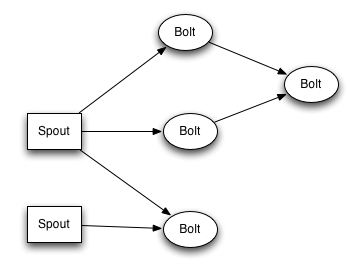
\includegraphics[scale=0.45]{img/topology.png}
        \caption{Storm structor}
        \label{topology}
    \end{center}
\end{figure}

\subsection{Usage}

\begin{itemize}
    \item Stream processing - 
    \item Distributed RPC
    \item Continous computation
\end{itemize}

\subsection{Simple Example}

\begin{code}
        builder.setSpout("RedditPostsReader", new RawRedditSpout());

        builder.setBolt("FilterPostString", new filterBolt()).shuffleGrouping("RedditPostsReader");
        builder.setBolt("", new ()).shuffleGrouping("");


\end{code}
\subsubsection*{Explanation}

\section{Online machine learning}

Online machine learning, is an induction model for learning from one instance at a time. This makes online algorithems perfect for data streams, since the model can be easily and constantly adjusted to acomodate for the newer data. As long as a good clasifier exists, the online algorithem will eventually learn to make better predictions. Online algorithems work with a sequence of trials, each of those can be represented with three steps. In the first step, the algorithm receives an instance, then in the second step, it predicts the label of the instance, and in the last step the algorithm receives the true label of the instance. The third step then also corrects the hypothesis to minimize the error, hopefully to make better predictions for future trials. 

One drawback of these algorithems, is the need for more and more correctly labeled examples from which the algorithem would learn. This ofcourse is not possible, when correctly labeling an example costs money and time. Fortunately there are a lot of problems where the correct label is always available. For example any problem that has to do with predicting the future. In those problems the label will eventually be available and the algorithem will be able adjust its model to compensate the new data. A case of a future prediction problem would be movements on the stock market, or finding the next trending topic on twitter.

A few popular online machine learning algorithems are \textit{perceptoron}, \textit{winnow} and \textit{naive bayes}. 

\subsection{Introduction}

\section{Machine learning with Storm}

As we have seen in the previous sections, Storm is a very powerful tool, used for a lot of different purposes. In this section, we will see implications Storm has in the data mining field. 

\subsection{preprocessing}
Storm topologies can be used for machine learning indirectly, just for data preprocessing before running the data on a machine learning algorithem. The most common use for this would be video analizing, image streams such as tumblr, or any other data type that needs preprocessing before any classification or regression can be done.

\subsection{prediction}
For this use case, Storm would act as distributed RPC that would just classify each instance from a given fixed model. 

\subsection{learning}

\section{Conclusion}

\appendices

\section*{Acknowledgement}
The authors would like to thank Matjaž Kukar, PhD Assistant Professor.


\begin{thebibliography}{1}
\bibitem{reservoir85}
J.~S. Vitter, \emph{Random Sampling with a Reservoir}. \relax Brown University, 1985.
\bibitem{learning}
N. Littlestone, \emph{Learning Quickly When Irrelevant Attributes
Abound: A New Linear-threshold Algorithm}. \relax University of California, 1988
\bibitem{auc}
P. Zhao, R. Jing, \emph{Online AUC Maximization} \relax School of Computer Engineering, Nanyang Technological Unoversoty \& Deparment of Computer Science and Engineering, Michigan State University
\bibitem{kessl}
R. Kessl, \emph{Parallel algorithms for mining of frequent itemsets} \relax The Faculty of Electrical Engineering, Czech Technical University in Prague
\bibitem{roc}Hanley, James A. and McNeil, Barbara J. \emph{The meaning and
use of the area under of receiver operating characteristic
(roc) curve.} \relax 1982.

\end{thebibliography}

\newpage

\begin{IEEEbiography}[{
\includegraphics[width=1in,height=1.25in,clip,keepaspectratio]{majcn}}]{Gregor Majcen}
63070199
\end{IEEEbiography}

% if you will not have a photo at all:
\begin{IEEEbiography}[{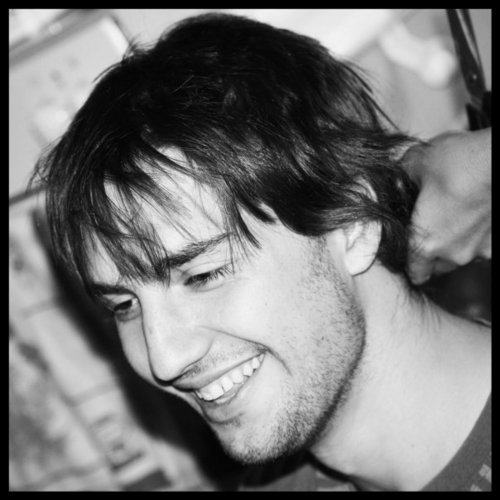
\includegraphics[width=1in,height=1.25in,clip,keepaspectratio]{zidar}}]{Miha Zidar}
63060317
\end{IEEEbiography}
\end{document}


